\chapter{Conclusiones y trabajo futuro}

\section{Mejoras}
Como todo software, siempre puede ser mejorado, y el presentado en este
TFG no es ninguna excepci\'on. El software puede mejorarse sobre todo en tres niveles 
bien diferenciados: Apariencia, dise\~no y funcionalidades, eso sin contar, por
supuesto, los bugs que no han sido descubiertos en la fase de testing y que
casi seguro surgir\'an durante su vida \'util en producci\'on.

Los puntos clave en los que creo que este software puede mejorarse es sobre todo
en dise\~no.

Por ejemplo, pese a que lo he hecho lo mejor que he podido y que he sabido,
seguro que en muchos puntos podr\'ia utilizarse SOLID de manera m\'as efectiva. Un
ejemplo claro de esto que digo es el uso del patr\'on Singleton. Tal y como he detallado
en el cap\'itulo de An\'alisis y dise\~no, muchos desarrolladores sostienen
que no es buena idea utilizarlo, ya que las dependencias est\'an en el c\'odigo,
no en las relaciones entre las clases. Una clase que utilice el patr\'on Singleton tiene
un \'ambito global y utilizar objetos globales para
no pasar la referencia de clase en clase est\'a considerado un 
\emph{code smell \footnote{\url{https://en.wikipedia.org/wiki/Code_smell}}
	 \footnote{Lista incompleta de smells: \url{http://blog.codinghorror.com/code-smells/}}}.

No s\'olo es un \emph{code smell} si no que adem\'as incumple el principio de responsabilidad \'unica de SOLID.
Y lo incumple porque la clase que utiliza el patr\'on tiene dos responsabilidades: Controlar que s\'olo exista
una \'unica instancia y adem\'as su propia l\'ogica de negocio.

Es por ello que una de las mejoras que propongo, es sustituir los Singleton por patrones
Factory o patrones Builder para que sea esa clase externa la que limite la creaci\'on de instancias.
De esta manera es m\'as escalable, ya que es muy probable que lo que hoy es \'unico, ma\~nana sea m\'ultiple.

Otra cosa que no se ha realizado, y que se considera una buena pr\'actica de programaci\'on son
las pruebas unitarias. Una vez implementadas podr\'ia utilizarse un enfoque m\'as del estilo
de XP \footnote{eXtreme Programming: \url{http://www.extremeprogramming.org/}}, esto es, que todo gire
en torno a las pruebas unitarias. Un bug no es un error, sino una prueba que no est\'a escrita. Y si esa 
prueba que no estaba escrita falla, entonces es que hay un requisito que no se est\'a cumpliendo.

Muy relacionado con las pruebas unitarias, es el TDD \footnote{Test Driven Development} en el cual no se programa
nada hasta que no se hayan escrito todas las pruebas. Y un software se considera terminado cuando todas las pruebas
validan. Obviamente hay que probar todas las situaciones posibles.

Otro de los \'ambitos que tiene mucho margen de mejora es el procesamiento paralelo. Si que es cierto que se ha
utilizado, pero las posibilidades que da son enormes, y no se ha utilizado m\'as que en dos casos
muy concretos. Con unas semanas de estudio y con algo de refactorizado del c\'odigo estoy seguro
que se le podr\'ia sacar mas partido a los m\'ultiples n\'ucleos de los ordenadores actuales.

Por otro lado, como la aplicaci\'on aqu\'i presentada, en un futuro ser\'a integrada dentro de un sistema m\'as grande,
requerir\'a de un poco de trabajo si no se quiere mantener como una aplicaci\'on independiente.
Para ello, habr\'ia que convertir \texttt{MainWindow} en una subclase de \texttt{UserControl}, para
que de esta manera pueda ser a\~nadido como una ventana acoplable al otro sistema.

Por \'ultimo en cuanto a temas de dise\~no se refiere, yo propongo cambiar los temporizadores de la
aplicaci\'on y utilizar los \emph{data bindings} que proporciona .NET. Para poder hacer esto
habr\'ia que aprender bien a utilizar el patr\'on MVVM, que si bien se ha utilizado en este proyecto
no se le ha exprimido todas las caracter\'isticas.

Finalmente, est\'eticamente hablando, yo considero que es una aplicaci\'on intuitiva, pero se podr\'ia conseguir
que todo fuera m\'as claro si los gr\'aficos entre observaciones no compartieran el mismo color,
es decir, si la observaci\'on 1, tiene los gr\'aficos de color verde, que la observaci\'on 2 los tenga de color azul.
Ya que as\'i, queda m\'as bonito al ojo, y es m\'as f\'acil no confundir a que observaci\'on pertenece cada propiedad.
Tambi\'en hay otra mejora cosm\'etica, y es que cuando el usuario haga doble click sobre un elemento del \'arbol
de propiedades y observaciones, si ese \'item ya estaba cargado, que cogiera el foco, en vez de no hacer nada, que 
es lo que hace actualmente. Y tambi\'en ser\'ia interesante crear un di\'alogo de opciones, ya que ahora las
opciones est\'an metidas dentro de un XML y hay que editarlo a mano.

\section{Conclusiones}
Para finalizar, en una memoria no puede faltar una secci\'on en la cual el desarrollador
hace una reflexi\'on sesuda sobre el trabajo realizado, que es lo que se planific\'o
y lo que ha sido realmente...

\subsection{Reflexiones}
Pues all\'a vamos. Empecemos por la reflexi\'on sesuda.
Con todo proyecto grande en el que me involucro me pasa siempre lo mismo, a lo que yo llamo
``el  s\'indrome del programador". B\'asicamente consiste en que da igual lo que hagas,
tu c\'odigo nunca va a ser lo suficientemente bueno, tu c\'odigo siempre va a necesitar
de nuevas funcionalidades, funcionalidades que ni siquiera se ped\'ian, pero como se le profesa
un ``cari\~no" \ especial al software, siempre se intenta mejorar, aunque sea con nimiedades.

Eso nos lleva a no centrarnos en las tareas principales, se tiende a no hacer el software que nos piden
sino, el software que el propio desarrollador querr\'ia si fuese el quien ha encargado dicho software.
Esto es algo muy peligroso, porque podemos meternos en un bucle de hacer/deshacer cosas \'epico, ya que
lo que hoy parece una idea brillante, ma\~nana se te ocurre una manera mejor de hacerlo, y siempre
se piensa que la nueva manera es \'optima. Pero nada mas lejos de la realidad. En muchas ocasiones el
cambio est\'a justificado, si se trata de refactorizar, mejorar dise\~no etc. Mi opini\'on es que \'unicamente
hay que cambiar algo que ya funciona cuando la mejora es visible. Es decir, que has cambiado un algoritmo O(n)
por uno O(1) u O(ln n)...

Este s\'indrome no afecta solo a la parte de dise\~no e implementaci\'on, sino tambi\'en a la interfaz gr\'afica:
``Es que si ponemos este bot\'on aqu\'i queda m\'as claro...", ``Si a\~nadimos una nueva ventana de opciones es m\'as
amigable con el usuario...". A lo que yo digo, si no se piden esos cambios, son bobadas. Porque primero, esos cambios
no te los van a pagar, y segundo, tal vez el cliente no los quiera y te toque deshacer el trabajo.

He de admitir que yo mismo he sufrido ese s\'indrome durante este proyecto, obsesion\'andome a ratos con tonter\'ias
que no afectaban al funcionamiento, que lo previo no pod\'ia considerarse que estuviera mal... Vamos, llegu\'e a cambiar
algoritmos enteros, sin mejorar su eficiencia simplemente porque pens\'e que el c\'odigo ser\'ia mas comprensible. Eso si,
sin olvidar que el c\'odigo previo tampoco es que fuera chapucero.

En otra situaci\'on en la que sufr\'i dicho problema, es cuando se implement\'o la funcionalidad de crear un intervalo
para despu\'es poder guardarlo a disco. Me pareci\'o muy interesante crear otro panel lateral en el que mostrar los intervalos 
que hab\'ian sido creados y que estaban en la lista de intervalos a exportar. Puede ser una buena idea, que a\'un sigo pensando
que merece la pena implementarlo, pero no era un requisito inicial, y adem\'as trae consigo otro tipo de implicaciones. 
Habr\'ia que mantener ese listado de alguna manera enlazado con la lista de los intervalos, si se muestra, tiene sentido
que puedan ser tanto editados, como borrados. A simple vista parece un a\~nadido f\'acil, pero no se sabe hasta que punto
puede llegar a modificar el comportamiento actual, y cuanto tiempo me llevar\'ia hacerlo, por lo que finalmente
fue descartado.

Por otro lado, una de las razones personales de elegir este TFG fue porque me obligaba a salir de mi zona
de confort. Habr\'ia sido muy f\'acil elegir un TFG que manejase materias que se me dieran bien
y me gustasen especialmente, tecnol\'ogicamente hablando. A mi no me gusta crear interfaces gr\'aficas,
y este TFG giraba sobre todo a un software con una interfaz gr\'afica compleja. Jam\'as hab\'ia trabajado
con WPF ni con las versiones nuevas de .NET. Pueden parecer que no es un cambio grande, pero hay un mundo de
diferencia entre Java y .NET, las cosas se hacen muy diferente aunque sint\'acticamente sean muy similares.

Tampoco hab\'ia usado nunca librer\'ias externas de gr\'aficos ni de distribuci\'on de ventanas. Ha sido
un proyecto que ha presentado muchos retos, situaciones en las que nunca hab\'ia trabajado previamente,
pero que creo que han sido resueltas de una manera bastante elegante y eficiente para ser
la primera vez que se trabajan con ellas. Eso si, es muy mejorable todo. Aparte
de no haber utilizado estas bibliotecas, est\'a el problema de que ninguna de las usadas
ten\'ia una documentaci\'on completa, por lo que se ha tenido que utilizar mucho los foros,
y realizar un poco prueba y error y navegando a trav\'es del propio c\'odigo
fuente de estas herramientas para ver como realizaban las cosas.

\subsection{Una historia de planificaciones y realidades}
No voy a ser yo quien diga que una planificaci\'on temporal es una herramienta in\'util.
Pero si voy a ser yo quien diga que trabajar en base a una planificaci\'on temporal es
un esfuerzo f\'util. Y m\'as si se trata de un software como el presentado
en este TFG.

A la gente que tiene un perfil tirando a gestor, y poco t\'ecnico, tiende a pensar
que en el mundo del software es f\'acil que la planificaci\'on y la realidad
vayan de la mano. Se equivocan, sobre todo cuando no est\'as haciendo un software propio,
si no que est\'as creando un software por encargo, donde los requisitos pueden
cambiar d\'ia si, y d\'ia tambi\'en. Se tiende a cometer el error de utilizar la planificaci\'on
temporal como una hoja de ruta inamovible, sin tener en cuenta la incertidumbre que rodea
a todo proyecto de software.

En mi caso concreto, seguir la planificaci\'on no ha sido un gran problema, ya que al tratarse
de sprints que conten\'ian a su vez varias tareas los cambios no son tan visibles.

Aun as\'i, puedo afirmar que las cosas han ido mejor de lo esperado, ya que este proyecto
ten\'ia un alto grado de incertidumbre al no conocer ni la plataforma de desarrollo, ni las
bibliotecas utilizadas, la mayor\'ia con documentaci\'on bastante deficiente.

En la Figura \ref{fig:burndown} se puede ver las tareas que me quedaban en cada iteraci\'on
y cual era el progreso ideal para acabarlo a tiempo. Tal y como se puede observar,
las dos l\'ineas no van ni mucho menos cerca.

Finalmente, aunque con un mes de retraso, el proyecto finaliz\'o satisfactoriamente.

\begin{figure}[h]
    \centering
    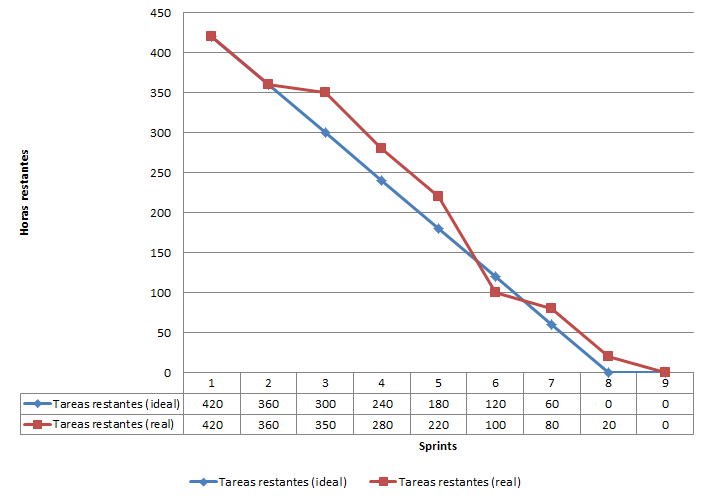
\includegraphics[width=0.8\linewidth]{./Figures/burndown.png}
    \caption{Burndown}
    \label{fig:burndown}
\end{figure}

Esto sirve para ver que aunque en algunos sprints se vaya con ``retraso", no implica que el proyecto
en general vaya con retraso. Porque a veces se va con retraso, y a veces se va adelantado.

En la planificaci\'on inicial se hablaba de que se iban a dedicar 60h/mes al proyecto,
pero finalmente no ha podido ser as\'i. Bien es verdad que ha habido situaciones en las
que se ha podido dedicar mas de 60h/mes, pero otras veces apenas se ha podido dedicar
unas escasas 20h/mes, por la carga de trabajo que hab\'ia durante las clases.

Tambi\'en me parece importante contar la experiencia que ha sido usar Scrum y Kanban. 
Seguir la metodolog\'ia de Scrum no ha sido muy complicado. Es cierto que no se ha aplicado
un Scrum de manual, ya que al ser un equipo de una persona, todas las tareas las realizaba la 
misma persona. Pese a todo, ha sido una manera de trabajar bajo mi punto de vista m\'as agradable,
ya que permite bastante flexibilidad. Y se ha hecho uso de esta flexibilidad en distintas ocasiones.
Por ejemplo cuando se a\~nadi\'o la funcionalidad de poder guardar m\'as de un intervalo en el mismo
XML, o cuando se a\~nadi\'o el \'arbol lateral con las observaciones y las propiedades.

En cambio, Kanban ha sido un poco mas dif\'icil de dominar. Normalmente en todos los sitios se insta
a que el trabajador no se quede quieto, ya que de esa manera deja de ser ``productivo". Por supuesto
esa manera de pensar, aunque yo personalmente est\'e de acuerdo, ha pesado mucho y 
muchas veces, cuando no se sab\'ia solventar un problema se tuvo la tentaci\'on de dejarlo de lado
y empezar con otra. En un par de ocasiones si que se realiz\'o eso mismo, pero estaba justificado
ya que requer\'ia la interacci\'on de una tercera persona. Tambi\'en fue complicado mantener
ordenado y actualizado el tablero Kanban. Este instrumento no s\'olo se utiliz\'o para gestionar
este TFG, si no para gestionar tambi\'en las tareas de clase. Finalmente se cogi\'o ritmo
y se cogi\'o la costumbre de que antes de ponerse a trabajar actualizar tanto el diagrama burndown
como el tablero Kanban. Ya que como se nos ense\~no en la asignatura de Sistemas de Gesti\'on Integradoss,
aquello que no se puede medir no se puede mejorar.

Y pese a coger esa costumbre sistem\'atica, fue imposible terminar el trabajo en el
plazo planificado. Podr\'ia decirse que hay excusa a la hora de entregar con retraso,
ya que una de las razones personales por las que eleg\'i este TFG era porque me
obligaba a salir de mi zona de confort como se ha comentado con anterioridad.